%!TEX root = ../thesis.tex
\chapter{Distilling the knowledge of pre-trained models} \label{ch:distillation}
\section{Overview}
Since the 2012 \textit{ImageNet} competition, many convolutional neural networks based architectures for computer vision have been proposed, leading to a large number of open source resources in the form of pre-trained models. In this chapter, the idea of combining the knowledge of multiple pre-trained models into another simpler pre-trained model using knowledge distillation techniques is studied. 

The experiments included in this chapter show improvements in the accuracy of the lightest pre-trained models when fine-tuning them using the soft-labels of their superior counterparts. The knowledge transfer is performed by using solely unlabeled data. Up to a 3.0\% and a 1.7\% absolute improvement in top-1 and top-5 accuracy is achieved across several models, suggesting that the trained architectures are still not at their capacity limit. This technique allows having a significant improvement of performance in mobile and other \textit{TinyML} applications \autocite{sanchez2020}.

 All the code used in this chapter is publicly available in a repository\footnote{\url{https://github.com/ivallesp/distillnet}}.

 \section{Introduction}
 Computer vision systems have evolved dramatically in the last decade due to the rise of deep learning technologies. In 2012, as described in chapter \ref{ch:background}, \textit{AlexNet} \autocite{krizhevsky2012} achieved the first position in the \textit{ImageNet} yearly challenge \autocite{ILSVRC15}, becoming the first neural network to get such position. Since then, the neural solutions prevailed, and many different architectures were proposed, each of them being better than the previous ones \autocite{khan2020, algan2021}. The parameters of many of the best deep learning models solving the \textit{ImageNet} problem are publicly available (e.g. \autocite{kaiming2016, chollet2017, szegedy2016, szegedy2017, howard2017, pham2018, tan2019}), in form of pre-trained models. One of the most common applications of pre-trained models is transfer learning \autocite{huang2021}, as briefly discussed in section \ref{sec:typesoflearning_others}, where the weights of a model  trained to solve a large scale task (commonly referred to as pretext task, such as the \textit{ImageNet} classification task) are re-utilized and fine-tuned to exploit them for another task. Usually, although not always, the first layers of the network are frozen and only the last few layers 
 are adjusted. This simple idea has been developed in the last years, and many further studies have been published (see \autocite{evci2022, zhu2018, wu2021, pzhao2021}). Transfer learning works under the hypothesis that lower layers learn simpler and widely applicable patterns that are used by higher level layers to solve the objective task.

 Another very powerful technique, named knowledge distillation, allows transferring knowledge from a teacher model to a student model. In 2015, a study showed that it is possible to improve the performance of a simple model (known as the student) by distilling the knowledge of a more sophisticated model (named the teacher) \autocite{hinton2015}. The technique proposed in the work of \textit{Hinton et al.} is very simple and consists on training the student with the soft-targets of the teacher, given a transfer dataset. The soft-targets are the raw predictions of the model, which are expressed as probabilities of belonging to each class. The authors suggest to minimize the cross-entropy with soft-targets, after dividing the logits by a temperature constant $T$ (process known as warming the logits, extra details in section \ref{sec:distillation_kd}) so that the probability distribution gets less sparse (i.e. more distributed across the classes that are different than the most probable class). This technique is built under the hypothesis that there is more information in the soft targets than in the hard targets (i.e. the labels). This additional information is sometimes known as \textit{dark knowledge} \autocite{gou2020}. Knowledge distillation is still a hot topic in nowadays research (see \autocite{tan2021, zhao2021, lee2021}).

  This work explores the following hypothesis: the performance of a small pre-trained model can be improved by leveraging the knowledge of one or multiple larger pre-trained models, while keeping the computational budget small and using solely unsupervised data. An ensemble of pre-trained models may be the most powerful solution in terms of performance but it is obviously energy-inefficient and may not be applicable for mobile applications, tasks that require a time-sensitive inference \autocite{sanchez2020} or other \textit{TinyML} tasks. Therefore, the problem is approached from a knowledge distillation perspective, with the aim to distill the knowledge of multiple heavy pre-trained models into a light-weight base model. The experiment results show that not only it is possible to improve its original accuracy but that some techniques for combining the knowledge of multiple teachers are better than others. 
  
There is a plethora of applications that can benefit from the results of this study. The first one is data intense applications such as video event detection \autocite{chakraborty2021}, for instance in autonomous driving \autocite{swaminathan2019}, where a large number of frames need to be processed in real time and with a high performance. The second one is tasks that need to run necessarily in a low-resource device, like a mobile device (e.g. augmented reality for map localization \autocite{limmer2017}), or the time-sensitive tasks (e.g. facial recognition for security \autocite{aung2021}). Finally, the proposed models are more environmental-friendly, as they require less energy for training and inference \autocite{wu2022sustainable}.


 \section{Previous work} \label{sec:distillation_prevwork}	
 A few previous studies have been published where the objective was to combine multiple deep learning models. The authors of \autocite{liu2020b} distill the knowledge of several teachers into a multitask student in the computational linguistics domain. Apart from the different domain of application, their approach differs from the one described in this chapter in the fact that their student and teachers goals differ: their student learns to combine the different objectives of the teachers. In \autocite{geyer2019}, the authors present a new technique that allows merging multiple models using a parameter fusing technique based on the incremental mode matching (IMM) procedure \autocite{lee2017}. This methodology has an important limitation that makes it unsuitable for this use case: the pre-trained and the target architecture must have the same structure. The objective is to improve the performance of a light-weight model using the knowledge of its greater siblings, which normally have more complex architectures. 
 
 In the work of \autocite{asif2019}, the authors define a framework to learn a small ensemble of students from a large ensemble of teachers which are combined linearly. For that, they propose to define a neural network architecture with as many student branches as teachers. The student branches are trained to minimize the \textit{Kullback-Leibler} (KL) divergence with their corresponding teacher branch, as well as minimizing the KL-divergence between the linear combination of the students, and the linear combination of the teachers. The approach proposed in this chapter differs fundamentally in the fact that the base architecture size of the proposal is independent of the number of teachers. In addition, instead of using KL-divergence losses, the cross-entropy with soft-targets is used, as defined by \autocite{hinton2015}.

 Additionally, multiple works have been found in the literature where the objective is to design lightweight convolutional neural networks for multiple tasks \autocite{zhou2020, jeon2021, hui2018}. Different techniques can be used to lighten up the high computational cost and memory requirements of the classical convolutional neural networks architectures. These techniques range from efficient modifications of the convolution operation, such as depthwise-separable convolutions \autocite{chollet2017}, squeeze operations \autocite{qiang2021} or dilated convolutions \autocite{Yu2016}, to higher level architecture design choices such as systematically balancing the size of the architecture building blocks \autocite{tan2019} or pyramidal feature extraction \autocite{Lin2017}, typically applied in object detection or optical flow inference. In this work, given the restriction of using publicly available student models pre-trained on \textit{ImageNet} dataset, the architecture design is limited to the current available choices, hence innovative architecture design is out of the scope of this work. However, the chosen student architectures feature various of the efficiency techniques discussed in the literature, such as 1x1 convolutions \autocite{szegedy2017}, depthwise-separable convolutions \autocite{chollet2017}, efficient model width, height and resolution scaling \autocite{tan2019}, and compression-expansion blocks \autocite{howard2017, sandler2018}, among others.
 
 \section{Methods} \label{sec:distillation_methods}
This section describes the training methods used as well as the knowledge distillation framework and the techniques employed to blend the predictions of different teachers.

 \subsection{Knowledge distillation} \label{sec:distillation_kd}
 The original knowledge distillation method, as defined by \autocite{hinton2015}, consists on using the $C$ class probabilities (known as soft-targets) produced by a machine learning model (named the teacher) as the training objective for another, often simpler, machine learning model (named the student). The probabilities of a deep learning model $\mathbf{p_i}$ (where $i \in \{1,...,C\}$) are normally calculated by applying the \textit{softmax} function over the logits vector $\mathbf{z_i}$ \autocite{Goodfellow2016}. Usually, a temperature parameter $T$ is introduced with the aim of producing a softer\footnote{Closer to a uniform distribution.} probability distribution over the classes (see equation \ref{eq:softmax}, where $i$ and $j$ represent class indices, and $t$ represents a specific teacher).

 \begin{equation}
 p_{i \in \{1 .. C\}} = \frac{\exp(z_{ti}/T)}{\sum_j^C \exp(z_{tj}/T)}
 \label{eq:softmax}
 \end{equation}

 The authors of \autocite{hinton2015} also recommend combining two loss functions: cross-entropy with soft-targets $\mathcal{L}_S$ and cross-entropy with hard-targets  $\mathcal{L}_H$. The first objective is computed with the probabilities of the student $p( \mathbf{z_s}, T)$ against the probabilities of a teacher model $p( \mathbf{z_t}, T)$, where the temperature $T$ is artificially increased to inflate the weight of the \textit{dark knowledge} \autocite{hinton2015}. The second objective is computed using  $T=1$ on the probabilities of the student $p( \mathbf{z_s}, T=1)$ against the ground-truth label $y$. See the losses definitions in equations \ref{eq:ced} and \ref{eq:ces}, where $\mathbf{z_t}$ and $\mathbf{z_s}$ denote the logits for the teacher and the student models, respectively, and $\mathbf{y}$ denotes the ground truth label. The losses are combined as shown in equation \ref{eq:loss_distillation}, where the $\alpha$ parameter is intended to balance between the two losses \autocite{gou2020}.

 \begin{equation}
 \mathcal{L}_S\left[p( \mathbf{z_t}, T), p(\mathbf{z_s}, T) \right] = -\sum_i p_i(z_{ti}, T) \log \left(p_i(z_{si}, T)\right)
 \label{eq:ced}
 \end{equation}

 \begin{equation}
 \mathcal{L}_{H}\left[\mathbf{y}, p(\mathbf{z_s}, T=1) \right] = -\sum_i y_i \log \left(p_i(z_{si})\right)
 \label{eq:ces}
 \end{equation}

 \begin{equation}
 \mathcal{L} = \alpha \mathcal{L}_S + (1-\alpha) \mathcal{L}_{H}
 \label{eq:loss_distillation}
 \end{equation}

Along all the chapter, $\alpha$ is set to $1$ given that only unlabeled data is used for training, and hence no hard targets are available.

 \subsection{Teachers blending methods} \label{sec:distillation_teachers_comb}
  Different models may produce harder or softer posterior probability distributions. In order to be able to successfully combine different teacher models for building the teacher signal that will be distilled into the student, the posterior probability distributions needs to be calibrated.

  The hardness or softness of a distribution can be controlled with the temperature parameter $T$ (see equation \ref{eq:softmax}). In this case, as different models have been combined to build the soft target signal, the temperature of each model has been chosen so that the average probability of the most probable class becomes $S$. Hence $S$ represents a hyperparameter that must be chosen before training. The term $s$ is used to denote a specific choice of $S$.  $T$ has been determined independently for each pre-trained model so that $S=s$, on average over the transfer dataset. The value of $T$ has been found using the bisection method\footnote{$T=1$ and $T=6$ are used as starting points for the bisection method}, given that the equation \ref{eq:softmax} is continuous in $T$.

  Once the probability distributions have been calibrated, the following techniques have been defined as teacher blending proposals. The term $\theta_n$ is used to denote the parameter set of the teacher $n$. 

  \begin{itemize}
	  \item \textit{Mean}: following the same idea of ensemble models \autocite{kuncheva2004}, averaging all the teachers probabilities is proposed as the simplest method to combine all teachers knowledge. This is done by computing the arithmetic mean across the set of $N$ teachers, for every instance $x$ and class $c$.
	  $$p_{\text{mean}}(x, c) = \frac{1}{N} \sum_{n=1}^N p(c | x, \theta_n)$$
	  \item \textit{Median}: with the idea of improving the mean blending method with robust statistics, the same calculation is repeated but using the median across the set of $N$ teachers, for every instance $x$ and class $c$. The result of this operation needs to be normalized so that the probabilities across the $C$ different classes sum to 1. $$p_{\text{median}}(x, c) = \frac{\text{median}_n\ p(c | x, \theta_n) }{ \sum_{k}^{C} \text{median}_n\  p(k | x, \theta_n)}  $$
	  \item \textit{Random}: randomly choosing the teacher that provides the soft-target for each training example, in expectation, should lead to the mean of the teachers predictions. However, given that stochastic gradient descent based optimizers are used, this method is included with the hypothesis that it will increase the variability of the gradients, potentially leading to a more robust exploration. For that, the class probabilities for each instance $x$ are selected from a random teacher $\hat{t}$. The randomization is recalculated after every training epoch.
	  $$\hat{t} \sim U(1, T) \rightarrow \mathbf{p_\text{random}}(x) = \mathbf{p_{\hat{t}}}(x)$$
	  \item \textit{Maximum correlation}: selecting the teacher that has the maximum correlation with the rest of teachers for a given training example will potentially lead to a more refined training signal. To account for that, the \textit{Pearson}'s correlation coefficient between all the possible pairs of teachers (correlation matrix) is calculated, for every training example. Then, the average of the correlation coefficients of every teacher with the rest is calculated, in order to determine to what degree that teacher ``agrees'' with the rest for that given training example. 
	  \item \textit{Minimum entropy}: the probability distributions of the teacher predictions for a given training example can be more or less spread. One possible interpretation of that phenomenon is that the higher the spread of the output classes distribution is, the lower the confidence of the model prediction will be. With that assumption in mind, the use of the \textit{Shannon} entropy is proposed as a measure of the spread (the higher the entropy, the closer the class distribution will be to a uniform distribution), and hence choose, for every training example, the teacher which class probability distribution has the lowest \textit{Shannon} entropy. That teacher will be the one that provides a more confident prediction, under the mentioned assumption.
  \end{itemize}

 The methods described above can be categorized in aggregative and selective techniques depending on their operating principle. The ``mean'' and ``median'' techniques are considered aggregative techniques because for a given training example $x_i$, they merge information from different teachers to get the final soft-target probabilities. The ``random'', ``maximum correlation'' and ``minimum entropy'' are categorized as selective techniques given that for a training example $x_i$, they just select which teacher provides the soft-target signal.  

 \subsection{Pre-trained models}
 Some of the pre-trained models included in the \textit{Keras} library for \textit{Python} \autocite{chollet2015keras} have been used for the experiments presented in this chapter. One model from each family has been selected, excluding the VGG family of models, in favour of more modern and efficient alternatives. A short description about each of those architectures is included below.
 
  In order to select the pre-trained models that will be used as students, a combination of the number of parameters and accuracy obtained on the transfer dataset (with the original model parameters) has been used. Further details, including the number of parameters and the computational cost of each model, are included in table \ref{table:models}.

 \begin{enumerate}
	 \item \textit{ResNet} \autocite{kaiming2016}: convolutional neural network with multiple blocks where the output of the $l^{th}$ layer is added to the output of the $(l+1)^{th}$. This structure is known as \textit{residual connection} (or \textit{skip connection}), and leads to the following transition: $x_{l+1} = H_{l+1}(x_{l}) + x_l$, where $H$ represents a convolutional layer. Described in the section \ref{sec:deepernn}.
		\item \textit{Inception ResNet} \autocite{szegedy2017}: introduction of the \textit{residual connection} structure from \autocite{kaiming2016} to the classical \textit{inception} convolutional neural network model, combined with several efficiency tricks. The \textit{inception} model is based on the idea of using different convolution operations (with different receptive field sizes and pooling operations) in every layer, and concatenating the result together. Additionally, before each regular 2D convolution, a 1x1 convolutional layer is introduced to reduce the number of operations (see figure \ref{fig:inception}). The authors of \autocite{lin2014} provide a deeper study on 1x1 convolutions.
	 \item \textit{DenseNet} \autocite{huang2017}: convolutional neural network inspired by the \textit{ResNet} model \autocite{kaiming2016} that introduces direct connections from every layer to all the subsequent ones leading to the following transition: $x_{l+1} = H_l([x_0, x_1, ... x_{l-1}])$. The square brackets in the previous expression mean concatenation.
	 \item \textit{NASNet} \autocite{pham2018}: convolutional neural network designed using neural architecture search (NAS) with reinforcement learning algorithms. The final architecture structure resembles to \textit{inception} \textit{ResNet}, but has been optimized to have a higher inductive bias.
	 \item \textit{Xception} \autocite{chollet2017}: convolutional architecture inspired in \textit{inceptionV3}  \autocite{szegedy2016} that features \textit{depthwise-separable convolutions} for higher computational efficiency.
	 \item \textit{MobileNet V1} and \textit{V2} \autocite{howard2017, sandler2018}: convolutional architecture designed to be efficient and scalable with the objective of being implemented into mobile devices. These networks feature \textit{depthwise-separable convolutions} for reducing the number of parameters, compression-expansion blocks and the introduction of two parameters $\alpha$ and $\rho$, to control the depth of the network and the input image resolution, respectively.
	 \item \textit{EfficientNet} \autocite{tan2019}: highly scalable convolutional architecture that attempts to tie the network depth, width and the input image resolution  together into a compound single parameter referred as $\phi$. The architecture of the base model (aka \textit{EfficientNet}) has been designed using neural architecture search (NAS) techniques.
 \end{enumerate}
 
 \begin{figure}[hbt]
 
  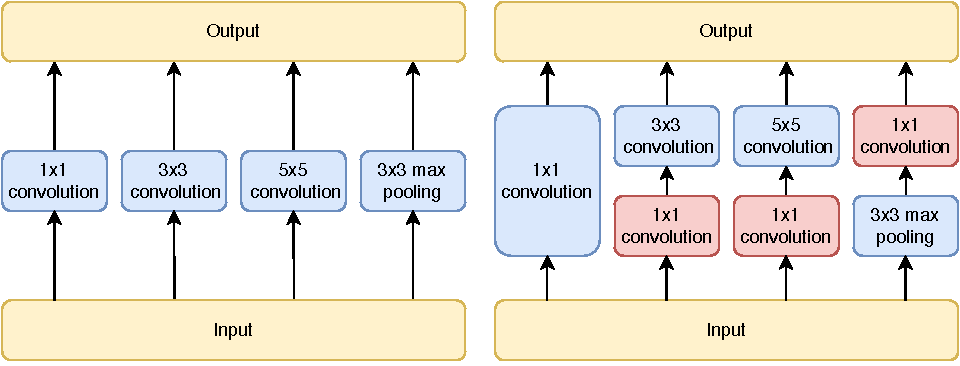
\includegraphics[width=1.0\linewidth]{./distillation/images/inception.pdf}
  \caption[Inception architecture building block]{Building block of inception architecture \autocite{szegedy2015}. Left: inception block without the dimensionality reduction trick. Right: inception block with convolutions 1D to reduce the total amount of operations.}
  \label{fig:inception}
\end{figure}


 \begin{table}[h]
	 \small
	 \caption[List of pre-trained models used in the experiments]{Pre-trained models used as teachers along this study, taken from \textit{Keras} implementations. Some of the input resolutions shown in the table may not correspond to the resolutions of the original papers, the models have been run in the resolutions indicated in the table as they showed a substantial performance improvement. The performance metrics reported in the table are empirical accuracies obtained by measuring the performance of the models against the \textit{ImageNet} 2012 validation dataset, using the \textit{Keras} implementations. They may differ from the performance reported in the original studies. $m$ means millions ($10^6$) and b means billions ($10^9$). The models that were used as students are formatted in bold.}
	 \centering
 \begin{tabular}{c|ccc|cc}
	 \toprule
			  Model          & Input size & \#Params &  FLOPs  & Top-1 acc. & Top-5 acc. \\ \midrule
		   NasNetLarge       &  331x331   &   89m    &  24b & 82.44\%  &  96.02\%    \\
		InceptionResNetV2    &  299x299   &   56m    & 13b & 80.44\%  &  95.31\%     \\
		\textbf{Xception}    &  299x299   &   23m    &  8.4b & 78.92\%  &  94.47\%     \\
		 EfficientNetB7      &  256x256   &   67m    &  37b & 77.88\%  &  93.87\%     \\
		   DenseNet201       &  256x256   &   20m    &  8.8b & 77.75\%  &  93.83\%     \\
		   DenseNet169       &  256x256   &   14m    & 6.7b & 76.60\%  &  93.39\%     \\
			ResNet50         &  256x256   &   26m    & 4.1b  & 75.53\%  &  92.53\%     \\
	  \textbf{DenseNet121}   &  256x256   &    8m    &  5.7b & 75.47\%  &  92.68\%     \\
	 \textbf{EfficientNetB0} &  256x256   &    5m    & 0.4b & 75.17\%  &  92.34\%     \\
	  \textbf{MobileNetV2}   &  256x256   &    4m    &  1.3b & 73.11\%  &  91.29\%     \\
		   MobileNetV1       &  256x256   &    4m    & 2.3b & 71.73\%  &  90.44\%     \\ \bottomrule
 \end{tabular}
 \label{table:models}
 \end{table}

 \section{Experiments and results} \label{sec:distillation_experiments}
This section provides an overview of the dataset that has been used in the experiments included in this chapter, describes the experiments performed and shows the results achieved.

 \subsection{Setup}
 The \textit{ILSVRC2012 ImageNet} dataset has been used in all the experiments \autocite{ILSVRC15}, given its large popularity and numerous available benchmarks. It is composed of 1.3 million images,  each of which belongs to only one class out of 1000 available classes. The data is provided in three separated subsets: train, validation and test, with 1.2M, 50,000 and 100,000 images in each set, respectively. The ground truth labels are provided for the train and validation sets, but not for the test set (i.e. the test set is unlabeled).

 The original dataset comes with images at different sizes and aspect ratios. Three different sets with the following sizes have been generated: 256x256, 299x299 and 331x331 (see table \ref{table:models} for the detailed model input sizes specifications). For that, first the images were resized so that their short edge matches the desired size and then center-cropping has been applied to get a square image, as it is common in these cases. Pixel values centering and scaling have been applied as per the functions provided with \textit{Keras} along with each pre-trained model. No data augmentation has been used along this study.

 In this work, the unlabeled test set is used as transfer dataset and the original validation set to measure and report performance (leaving $5\%$ out of the latter for development purposes).

Several experiments have been conducted to prove that the methodology described in this chapter scales to different settings. In those experiments, the following factors have been varied:

 \begin{itemize}
	 \item \textit{Student}: different small models are used as students to analyze how the methodology works with different students. The models used as students are: \textit{EfficientNetB0}, \textit{MobileNetV2}, \textit{DenseNet121} and \textit{Xception}. The reason those models are chosen as students and not the strictly smallest models is to favour variability in the architectures (e.g. MobileNetV1 and MobileNetV2 are very similar architectures, so only one of them was chosen).
	 \item \textit{Teachers set}: according to the performance shown in table \ref{table:models}, different sets of teachers are selected to build the distillation target: the ``best'' teacher (i.e. \textit{NasNetLarge}), the ``3-best'' teachers (i.e. \textit{NasNetLarge}, \textit{InceptionResNetV2} and \textit{Xception}) and ``all'' the 11 teachers.
	 \item \textit{Teachers blending methods}: the different sets of teachers are combined with the methods described in the section \ref{sec:distillation_teachers_comb}. These methods are referred in the tables below as ``mean'', ``median'', ``random'', ``maximum correlation'' and ``minimum entropy''. In the results section, the ``best'' teacher set is treated as a blending method\footnote{indeed, it can be seen as a special case of a selective blending method where the best teacher model is always selected}, to facilitate the reader to compare how different blending methods compare with just taking the best teacher as target (i.e. the \textit{NasNetLarge} model). 
 \end{itemize}

 The set of experiments conducted in this study is represented in the schema of figure \ref{fig:schema}.

\begin{figure}[h!]
 \centering
 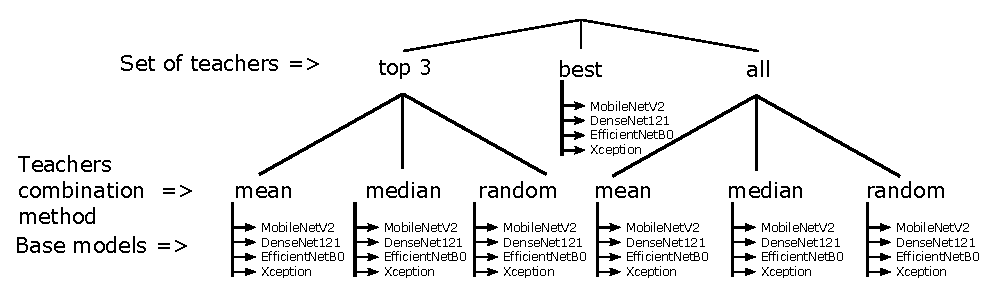
\includegraphics[width=0.6\linewidth]{distillation/images/schema}
 \caption[Distillation expriments summary schema]{Schema representing the combination of techniques tested in this study.}
 \label{fig:schema}
\end{figure}


Each experiment has been repeated 5 times to add more robustness to the results, totalling to 220 trained models. The students' initial weights have always been fixed to the pre-trained weights for the \textit{ImageNet} classification task, across all the experiments. During training, no layers have been frozen, allowing the optimizer to fine-tune all the weights in the student network. The temperature of the softmax in the output of the last layer has been increased in all the cases to match the normalized soft-targets distribution, as described in section \ref{sec:distillation_teachers_comb}.  Each model has been trained for 100 epochs, and the results are presented in the next section at the early stopping point (as per its performance in the development set). An \textit{Adam} optimizer \autocite{kingma14} and a learning rate of $10^{-6}$ have been used along all the experiments.

  In the experiments the hyperparameter $S=0.35$ is fixed, and the value of $T$ is determined for every pre-trained model using the bisection method with the transfer dataset. This value of $S$ has been chosen so that it produces an average temperature across the models of 2.0, which is close to the range recommended in \autocite{hinton2015}. Doubling the temperature parameter showed no noticeable improvements.

  To run the experiments, a single \textit{Nvidia RTX 2080ti} GPU has been used, and the code has been implemented in \textit{Tensorflow 2.0}.

 \subsection{Results}  \label{sec:distillation_results}
 Table \ref{tab:results1} summarize the results achieved by each of the experiments run over the \textit{ImageNet} dataset. The metrics reported are the top-1 accuracy and the top-5 accuracy, as it is standard in \textit{ImageNet} benchmarks, at the early stopping epoch. The results are expressed as the average metric $\pm$ the standard error.

 As it can be seen in the table, the proposed methodology achieves an absolute accuracy increase over the student's original top-1 accuracy of up to +3.10\%, +1.01\%, +0.97\% and +0.38\% for the \textit{EfficientNetB0}, \textit{MobileNetV2},  \textit{DenseNet} and \textit{Xception} students, respectively.
 % TODO: revise this numbers
 
The experiments showed that building a teacher signal by combining ``all'' the pre-trained models, or combining the ``3-best'' ones, leads to similar results. However, in some cases the results of distilling the combination of ``all' the teachers is superior than the ``3-best'' (e.g. \textit{DenseNet121} as student), but also the contrary occurs (e.g. \textit{EfficientNetB0} as student). Additionally, using only the ``best'' model as teacher often leads to overfitting issue, as it can be seen in figure \ref{fig:accuracycurves} (notice how the accuracy quickly degrades after reaching the maximum).

 Regarding the teacher combination method, the results show that the ``median'' method gets, in general, worse results than the ``mean'' method. Besides, the ``min entropy'' method achieves many of the best results when applied over the 3-best teachers (in 3 out of 4 student models as per the top-1 accuracy), but it is the winner blending method only once when applied with ``all'' the teachers. The results of the ``max correlation'' method, although they are superior to the original performance and competitive with the other methods, they do not seem to work as well as other methods. The techniques that better perform are the ``min entropy'' blending method followed by the ``mean'' blending method (both of them being the winner methods in 7 out of 8 teachers set and students combinations, as per top-1 accuracy).


Figure \ref{fig:accuracycurves}  shows the training curves for all the cases. As it can be seen in the figure, there are models for which the accuracy degrades more than the others after reaching the maximum accuracy (for instance this is the general trend of the ``best'' teacher). 

Choosing a very small learning rate was crucial to achieve the performance reported. Higher learning rates ($10^{-5}$ and  $10^{-3}$) were tested leading to worse performances (sometimes even worse than the original pre-trained model). However no exhaustive studies are performed around learning rate sensitivity due to the high resource requirements involved. This effect can be explained by the presence of catastrophic forgetting \autocite{French99}, which leads to overfitting to the transfer set when the learning rate is too large. The results are expressed as the average metric $\pm$ the standard error across the five repeated experiments.

 \begin{table}[h!]
  \tiny
 \centering
 \setlength{\tabcolsep}{4pt}
 \caption[Accuracy results of the distillation expriments]{Results in top-1 and top-5 accuracy (\%) for all the experiments. Each column in the table represents a different teacher set. The experiment that achieved the best performance for each student is highlighted in bold, a star symbol is added $\star$ in case the difference is significant with respect to the original accuracy with $\alpha=0.05$ (as per a one-sided one-sample t-test conducted separately for the Top-1 and Top-5 accuracy results). A second star symbol highlights the experiments that significantly beat the distillation with the best teacher (as per a one-sided two-samples t-test with $\alpha=0.05$)}.
 \begin{tabularx}{\textwidth}{XX|YY|YY}
	 \toprule
									&                          &                     \multicolumn{2}{c}{Top 1 accuracy}                      & \multicolumn{2}{|c}{Top 5 accuracy}                                       \\
	 Student \newline (Orig accuracy) & Blending\newline  method & \  \newline 3-best teachers          & \  \newline  all teachers            & \  \newline        3-best teachers  & \  \newline          all teachers   \\ \midrule
	 { EfficientNetB0}              & Best                     & $ 78.14 \pm 0.02 \star$              & $\mathbf{78.14 \pm 0.02 \star}$      & $94.17 \pm 0.00\star $              & $\mathbf{94.17 \pm 0.00\star} $     \\
	 (top1: 75.17)                    & Mean                     & $78.20 \pm 0.02 \star\star$          & $78.07 \pm 0.01 \star$               & $\mathbf{94.17 \pm 0.01}\star$      & $94.01 \pm 0.00\star$               \\
	 (top5:  92.34)                   & Median                   & $78.18 \pm 0.01 \star\star$          & $77.98 \pm 0.01 \star$               & $94.10 \pm 0.01\star$               & $93.93 \pm 0.01\star$               \\
									& Random                   & $78.21 \pm 0.01 \star\star$          & $78.05 \pm 0.01 \star$               & $94.08 \pm 0.01\star$               & $93.99 \pm 0.01\star$               \\
									& Min Entropy              & $\mathbf{78.27\pm0.01\star\star}$    & $77.94\pm0.01\star$                  & $94.16\pm0.01\star$                 & $94.07\pm0.01\star$                 \\
									& Max Correl.              & $78.18\pm 0.02\star$                 & $77.79\pm0.01\star$                  & $94.13\pm0.01\star$                 & $93.89\pm0.01\star$                 \\
									&                          &                                      &                                      &                                     &                                     \\
	 { MobileNetV2}                 & Best                     & $73.85 \pm 0.01 \star$               & $73.85 \pm 0.01 \star$               & $91.83 \pm 0.01\star$               & $91.83 \pm 0.01\star$               \\
	 (top1: 73.11)                    & Mean                     & $73.99 \pm 0.01 \star\star$          & $\mathbf{74.11 \pm 0.02} \star\star$ & $91.86 \pm 0.01\star\star$          & $\mathbf{92.02 \pm 0.01\star\star}$ \\
	 (top5: 91.29)                    & Median                   & $73.92 \pm 0.00\star\star $          & $74.04 \pm 0.01 \star\star$          & $91.84 \pm 0.01\star$               & $91.91 \pm 0.01\star\star$          \\
									& Random                   & $73.96 \pm 0.01 \star\star$          & $74.03 \pm 0.01\star\star$           & $\mathbf{91.88 \pm 0.00\star\star}$ & $91.96 \pm 0.01\star\star$          \\
									& Min Entropy              & $\mathbf{74.12\pm0.01\star\star}$    & $73.91\pm0.02\star\star$             & $91.87\pm0.01\star\star$            & $91.84\pm0.01\star$                 \\
									& Max Correl.              & $73.94\pm0.01\star\star$             & $73.84\pm0.01\star$                  & $91.78\pm0.01\star$                 & $91.77\pm0.01\star$                 \\
									&                          &                                      &                                      &                                     &                                     \\
	 { DenseNet121}                 & Best                     & $ 75.83 \pm 0.01 \star$              & $ 75.83 \pm 0.01 \star$              & $92.95 \pm 0.01\star$               & $92.95 \pm 0.01 \star$              \\
	 (top1: 75.47)                    & Mean                     & $75.92 \pm 0.01 \star\star$          & $\mathbf{76.44 \pm 0.02} \star\star$ & $93.04 \pm 0.01\star\star$          & $93.30 \pm 0.01\star\star$          \\
	 (top5: 92.68)                    & Median                   & $ 75.87 \pm 0.02 \star$              & $ 76.42 \pm 0.02 \star\star$         & $92.98 \pm 0.01\star\star$          & $93.29 \pm 0.01\star\star$          \\
									& Random                   & $75.92 \pm 0.02 \star\star$          & $76.43 \pm 0.01 \star\star$          & $93.03 \pm 0.01\star\star$          & $93.30 \pm 0.01\star\star$          \\
									& Min Entropy              & $\mathbf{76.00\pm0.01\star\star}$    & $76.09\pm0.01\star\star$             & $\mathbf{93.10\pm0.01\star\star}$   & $\mathbf{93.27\pm0.01\star\star}$   \\
									& Max Correl.              & $75.84\pm0.02\star$                  & $76.21\pm0.02\star\star$             & $92.96\pm0.01\star$                 & $93.20\pm0.02\star\star$            \\
									&                          &                                      &                                      &                                     &                                     \\
	 { Xception}                    & Best                     & $79.11 \pm 0.01 \star$               & $79.11 \pm 0.01 \star$               & $94.55 \pm 0.01\star$               & $94.55 \pm 0.01\star$               \\
	 (top1: 78.92)                    & Mean                     & $\mathbf{79.30 \pm 0.02} \star\star$ & $79.16 \pm 0.02 \star\star$          & $\mathbf{94.70 \pm 0.01}\star\star$ & $94.65 \pm 0.00\star\star$          \\
	 (top5: 94.47)                    & Median                   & $79.18 \pm 0.01 \star\star$          & $\mathbf{79.19 \pm 0.01 \star\star}$ & $94.65 \pm 0.01\star\star$          & $94.63 \pm 0.01\star\star$          \\
									& Random                   & $79.27 \pm 0.02 \star\star$          & $79.14\pm 0.01 \star\star$           & $94.68 \pm 0.01\star\star$          & $94.59 \pm 0.01\star\star$          \\
									& Min Entropy              & $79.31\pm0.02\star\star$             & $\mathbf{79.17\pm0.01\star\star}$    & $94.64\pm0.01\star\star$            & $\mathbf{94.69\pm0.01\star\star}$   \\
									& Max Correl.              & $79.19\pm0.01\star\star$             & $78.82\pm0.01$                       & $94.58\pm0.00\star\star$            & $94.44\pm0.00$                      \\ \bottomrule
 \end{tabularx}
\label{tab:results1}


 \end{table}



 \begin{figure}[h!]
	 \centering
	 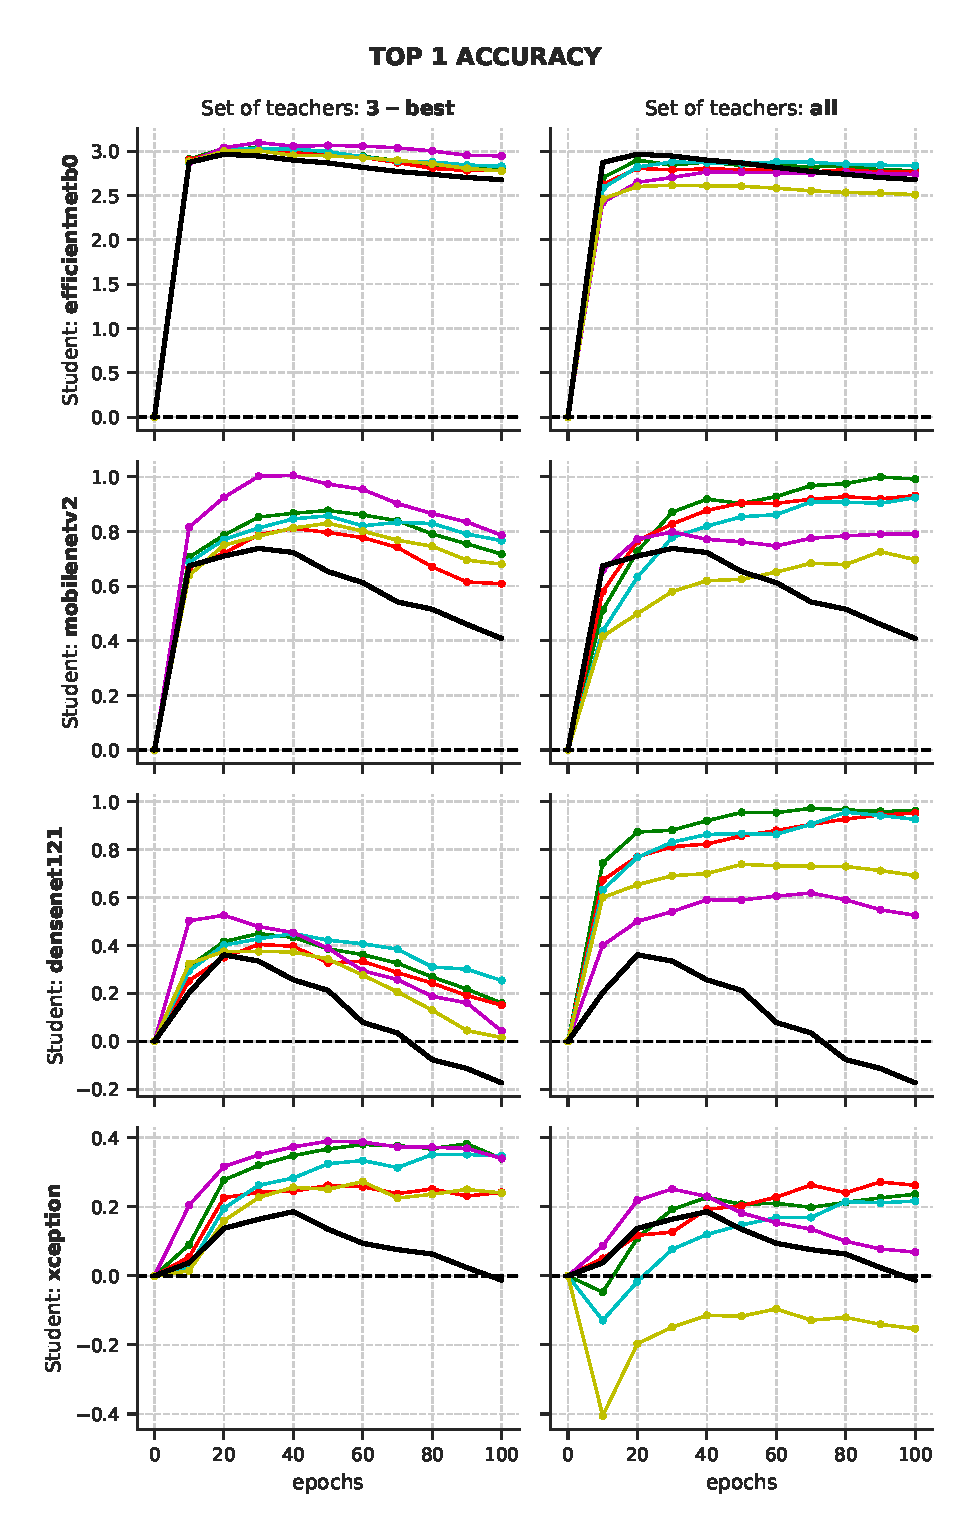
\includegraphics[width=0.475\linewidth]{distillation/images/top1_accuracy}
	 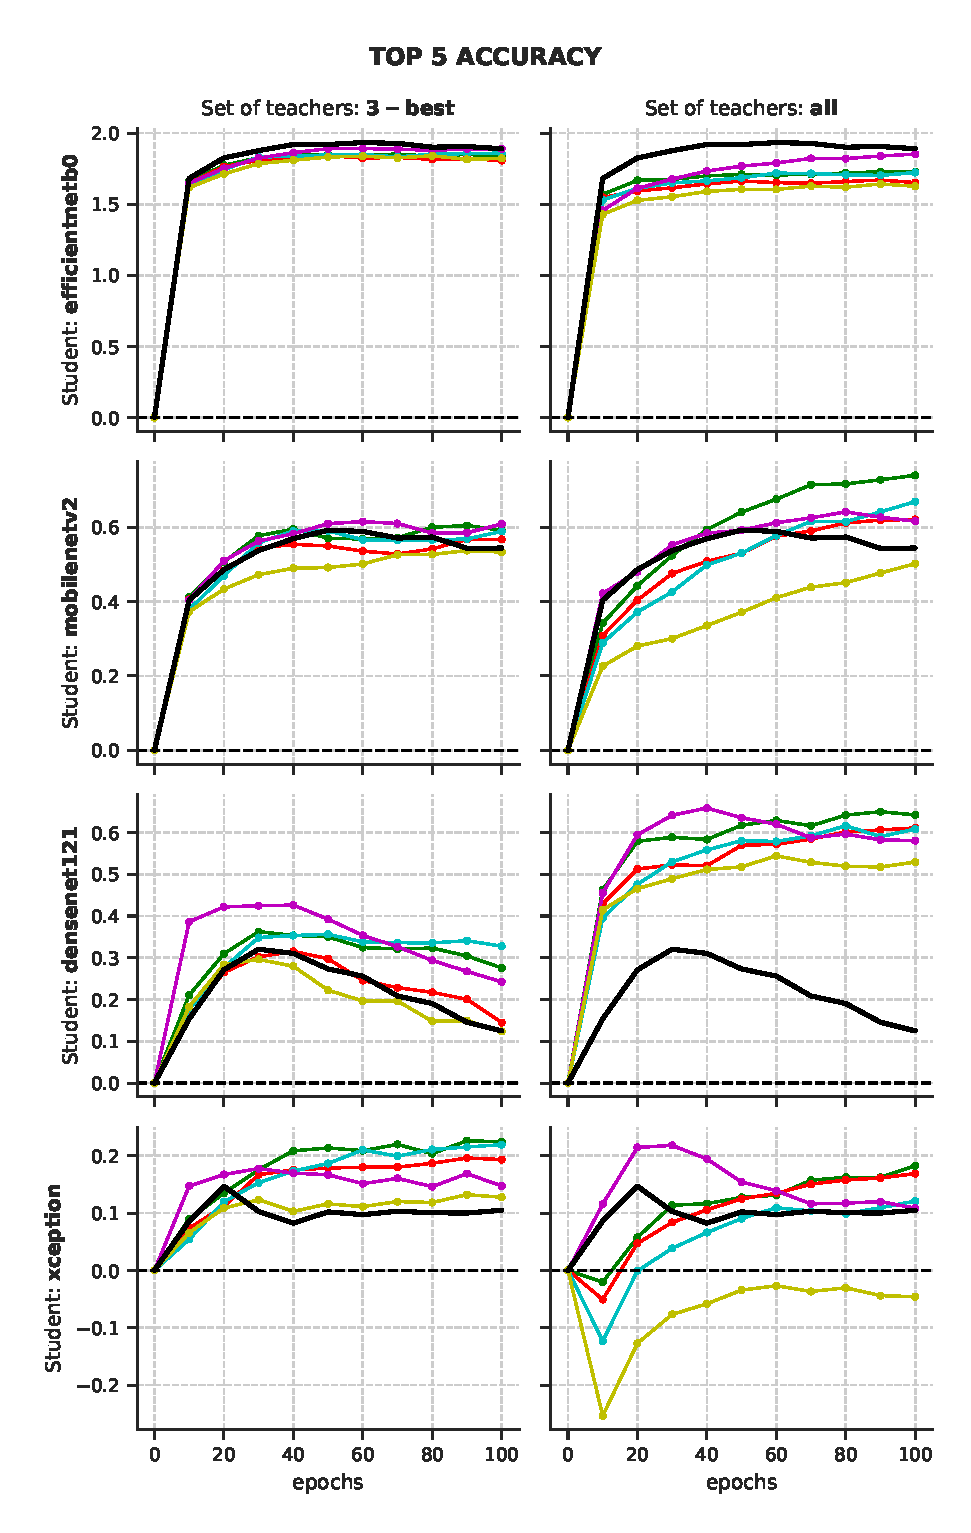
\includegraphics[width=0.475\linewidth]{distillation/images/top5_accuracy}
	 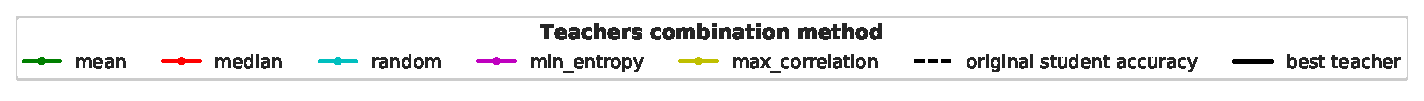
\includegraphics[width=0.95\linewidth]{distillation/images/legend}
	 \caption[Training curves of the distillation processes]{Absolute difference of top-1 accuracy (left) and top-5 accuracy (right) with respect to the baseline. The x-axis represents the number of training epochs, and the y-axis shows the absolute difference in performance with respect to the baseline. Each row in the grid represents a different student model. For comparison purposes, the training curve of the student trained by distilling the knowledge of the best teacher is included as a black line.}
	 \label{fig:accuracycurves}
 \end{figure}
 
 Finally, the accuracy increase depends substantially on the model being used as student, where the smaller student models are the ones that show the greatest accuracy increases.
 
 \subsubsection{Challenging the initial assumptions}
 With the aim of de-biasing the initial assumptions and gaining a better understanding of the dynamics of the proposed methods, this section includes the results of combining the teachers with the ``minimum correlation'' and with the ``maximum entropy'' methods (as opposed to the ``maximum correlation'' and ``minimum entropy'' methods described in section \ref{sec:distillation_methods}). The results are summarized in table \ref{tab:results2}, which shows that in the vast majority of cases the original definition gets significantly higher accuracy than the opposite case. This observation demonstrates that the assumptions taken upon the original methods definitions were accurate. The training curves of these experiments can be seen in figure \ref{fig:accuracycurves_challenging_assumptions}, included in the appendix.
 


 \subsection{Discussion}  \label{sec:distillation_discussion}
This chapter shows how it is possible to improve current low-resource pre-trained models by fine-tuning them on larger teacher soft-targets. This is, presumably, the first work that attempts to apply knowledge distillation techniques to pre-trained models. The aforementioned observations lead to the following conclusions: (1) the smaller the student model, the higher the accuracy increase, (2) increasing the number of teachers often leads to more stable training process, reducing the overfitting, and (3) the ``min entropy'' and the ``mean'' teacher blending methods often show significantly superior results compared to the rest of methods.
 
 Smaller pre-trained models generally have lower performance than their larger counterparts. This is due, among other possible reasons, to the fact that smaller models have less modeling capacity. Consequently, smaller models have the highest performance gap with the larger pre-trained models, and this has a strong implication in conclusion (1). If the performance gap between the original student model and the teacher signal is large, the student has a larger room for improvement, and hence the observed accuracy increase is larger.
 
 In conclusion (2), distilling the knowledge of multiple teachers often leads to better results than using a single one.  The intuition behind that observation is that the variability in the soft-targets increases as more models are combined, and that increases the amount of \textit{dark knowledge}, helping the student model reach a better solution. 
 
 In addition, from the training curves of figure \ref{fig:accuracycurves}, it can be concluded that the training processes of the experiments that use larger sets of teachers seem to be more robust, in the sense that the accuracy does not quickly degrade after reaching the maximum accuracy. The hypothesis behind this phenomenon is that when several teachers are combined to build the distillation target, the complexity of the classification task increases and that has, in essence, a regularization effect.
 
 \begin{table}[h]
	 \tiny. 
	 \centering
	 \setlength{\tabcolsep}{3pt}
	 \caption[Results of the min/max entropy and correlation methods]{Results in top-1 and top-5 accuracy (\%) comparing the original ``min entropy'' and ``max correlation'' methods with their opposite counterparts. In each comparison, the method that achieved the maximum accuracy is highlighted in bold, and a star symbol $\star$ is added where the difference was statistically significant with $\alpha=0.05$ (as per a one-sided two-sampled t-test).}
	 \begin{tabularx}{\textwidth}{rr|YY|YY}
		 \toprule
						   &                         &              \multicolumn{2}{c}{Top 1 accuracy}              & \multicolumn{2}{|c}{Top 5 accuracy}                                    \\
				   Student &        Blending  method & \  \newline best-3 teachers   & \  \newline  all teachers    & \  \newline        best-3 teachers & \  \newline          all teachers \\ \midrule
		 { EfficientNetB0} &  Min Entropy (original) & $\mathbf{78.27\pm0.01\star}$  & $\mathbf{77.94\pm0.01\star}$ & $\mathbf{94.16\pm0.01\star}$       & $\mathbf{94.07\pm0.01\star}$      \\
						   &  Max Entropy (opposite) & $78.0\pm0.01$                 & $77.56\pm0.02$               & $94.0\pm0.01$                      & $93.75\pm0.00$                    \\
						   &  Max Correl. (original) & $\mathbf{78.18\pm 0.02\star}$ & $\mathbf{77.79\pm0.01\star}$ & $\mathbf{94.13\pm0.01\star}$       & $\mathbf{93.89\pm0.01\star}$      \\
						   &  Min Correl. (opposite) & $78.07\pm0.02$                & $77.26\pm0.01$               & $94.08\pm0.01$                     & $93.66\pm0.01$                    \\
						   &                         &                               &                              &                                    &                                   \\
			{ MobileNetV2} &  Min Entropy (original) & $\mathbf{74.12\pm0.01\star}$  & $\mathbf{73.91\pm0.02\star}$ & $\mathbf{91.87\pm0.01\star}$       & $\mathbf{91.84\pm0.01\star}$      \\
						   &  Max Entropy (opposite) & $73.69\pm0.01$                & $73.38\pm0.02 $              & $91.65\pm0.01$                     & $91.44\pm0.01$                    \\
						   &  Max Correl. (original) & $\mathbf{73.94\pm0.01\star}$  & $\mathbf{73.84\pm0.01\star}$ & $\mathbf{91.78\pm0.01}$       & $\mathbf{91.77\pm0.01\star}$      \\
						   &  Min Correl. (opposite) & $73.83\pm0.01$                & $72.57\pm0.01	$              & $91.77\pm0.02$                     & $91.29\pm0.01$                    \\
						   &                         &                               &                              &                                    &                                   \\
			{ DenseNet121} & Min Entropy  (original) & $\mathbf{76.00\pm0.01\star}$  & $\mathbf{76.09\pm0.01\star}$ & $\mathbf{93.10\pm0.01\star}$       & $\mathbf{93.27\pm0.01\star}$      \\
						   & Max Entropy  (opposite) & $75.55\pm0.02$                & $75.49\pm0.02$               & $92.8\pm0.01$                      & $92.86\pm0.01$                    \\
						   &  Max Correl. (original) & $\mathbf{75.84\pm0.02\star}$  & $\mathbf{76.21\pm0.02\star}$ & $\mathbf{92.96\pm0.01}$       & $\mathbf{93.20\pm0.02\star}$      \\
						   & Min Correl.  (opposite) & $75.66\pm0.01$                & $75.29\pm0.02$               & $92.94\pm0.01$                     & $92.83\pm0.01$                    \\
						   &                         &                               &                              &                                    &                                   \\
			   { Xception} & Min Entropy  (original) & $\mathbf{79.31\pm0.02\star}$  & $\mathbf{79.17\pm0.01\star}$ & $\mathbf{94.64\pm0.01\star}$       & $\mathbf{94.69\pm0.01\star}$      \\
						   & Max Entropy  (opposite) & $78.78\pm0.02$                & $78.40\pm0.01$               & $94.46\pm0.01$                     & $94.16\pm0.01$                    \\
						   & Max Correl.  (original) & $\mathbf{79.19\pm0.01\star}$  & $\mathbf{78.82\pm0.01\star}$ & $\mathbf{94.58\pm0.00\star}$       & $\mathbf{94.44\pm0.00\star}$      \\
						   & Min Correl.  (opposite) & $78.76\pm0.02$                & $77.45\pm0.02$               & $94.44\pm0.01$                     & $93.82\pm0.0$                     \\ \bottomrule
	 \end{tabularx}
	 \label{tab:results2}
 \end{table}
 
 Another important observation is that the standard error of the results is very small (see table \ref{tab:results1}) because the initial weights in each student are the same across the 5 repetitions: the weights of the pre-trained model. The variability reported is produced by stochastic processes other than the initialization, such as dropout, the mini-batches arrangement, or the random teacher selection.

 In conclusion (3), the ``min entropy'' and the ``mean'' methods seem to be the ones producing the best results more often. Also, the ``median'' and ``max correlation'' methods do not perform as well as the rest. In the ``median'' case, this may be happening because, when using this blending method to combine the teacher predictions, the probability distribution is not preserved (i.e. the output probabilities for every class do not sum to 1),  having to apply a posterior renormalization step. This process may add some noise to the new distillation target. However, it is not clear why the ``max correlation'' method is not as good as the rest of methods.   
 
 %TODO: Find reasons why max_correlation is not a good method, and why mean and min_entropy are. 
 
The results reported by this study are relevant given that the methods described are able to increase the performance of pre-trained models, leading to classifiers with significantly higher performance for the same computational budget.   For instance, it was shown that by distilling the knowledge of the \textit{3-best} teachers into the \textit{EfficientNetB0} student using the ``random'' teachers combination method (one of the best results achieved, as shown in table \ref{tab:results1}), the student ends up performing better than the \textit{EfficientNetB7}, as per the top-1 accuracy (see table \ref{table:models}), while only requiring less than 7.5\% of the parameters and 1.05\% of the computation (around $100\times$ fewer FLOPs) than \textit{EfficientNetB7} \autocite{tan2019}.
 
 The training process described on this study is also advantageous from the computational standpoint. The \textit{ImageNet} training dataset is roughly $12.8\times$ larger than the transfer dataset used to fine-tune the students. Additionally, the number of \textit{FLOPs} of the students is, on average, $3.5\times$ smaller than the teachers'. The compound effect of needing less data to train and having less computationally intensive models, leads to a process that needs $3.5 \cdot 12.8 = 44.8\times$ less computation. This means that provided with same-size batch sizes and the same number of training steps, the training process of the teachers would need, on average, about $44.8\times$ more operations than the students fine-tuning. 
 
 \section{Conclusions}  \label{sec:distillation_conclusions}
The experiments of this chapter show how by using simple knowledge distillation techniques, the accuracy of the smallest pre-trained models increase in just few training epochs. This discovery opens potential new research lines towards more sophisticated teacher blending techniques or distillation methodologies. This can also motivate the research of novel training techniques, alternative or complementary to \textit{backpropagation} given that, as empirically demonstrated, the pre-trained models still did not reach their maximum capacity.


 
 \section{Appendix}
 This section includes the training curves for comparing the ``min entropy'' and ``max correlation'' methods with their opposite counterparts.
	 % TODO: \usepackage{graphicx} required
 \begin{figure}[h!]
	 \centering
	 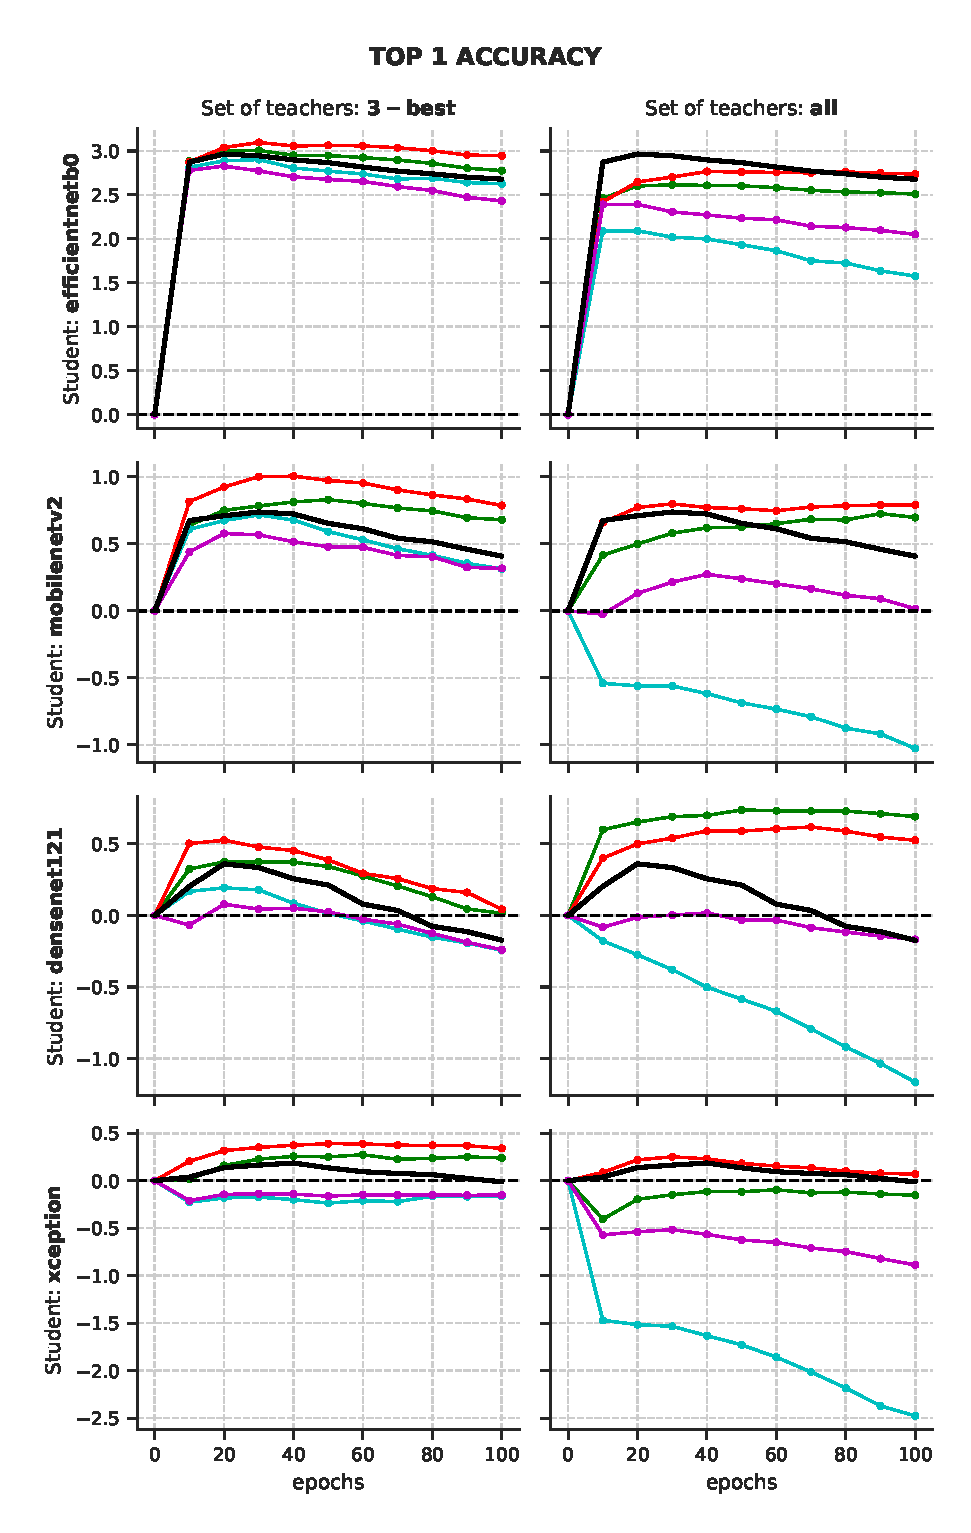
\includegraphics[width=0.475\linewidth]{distillation/images/top1_accuracy_challenging_assumptions}
	 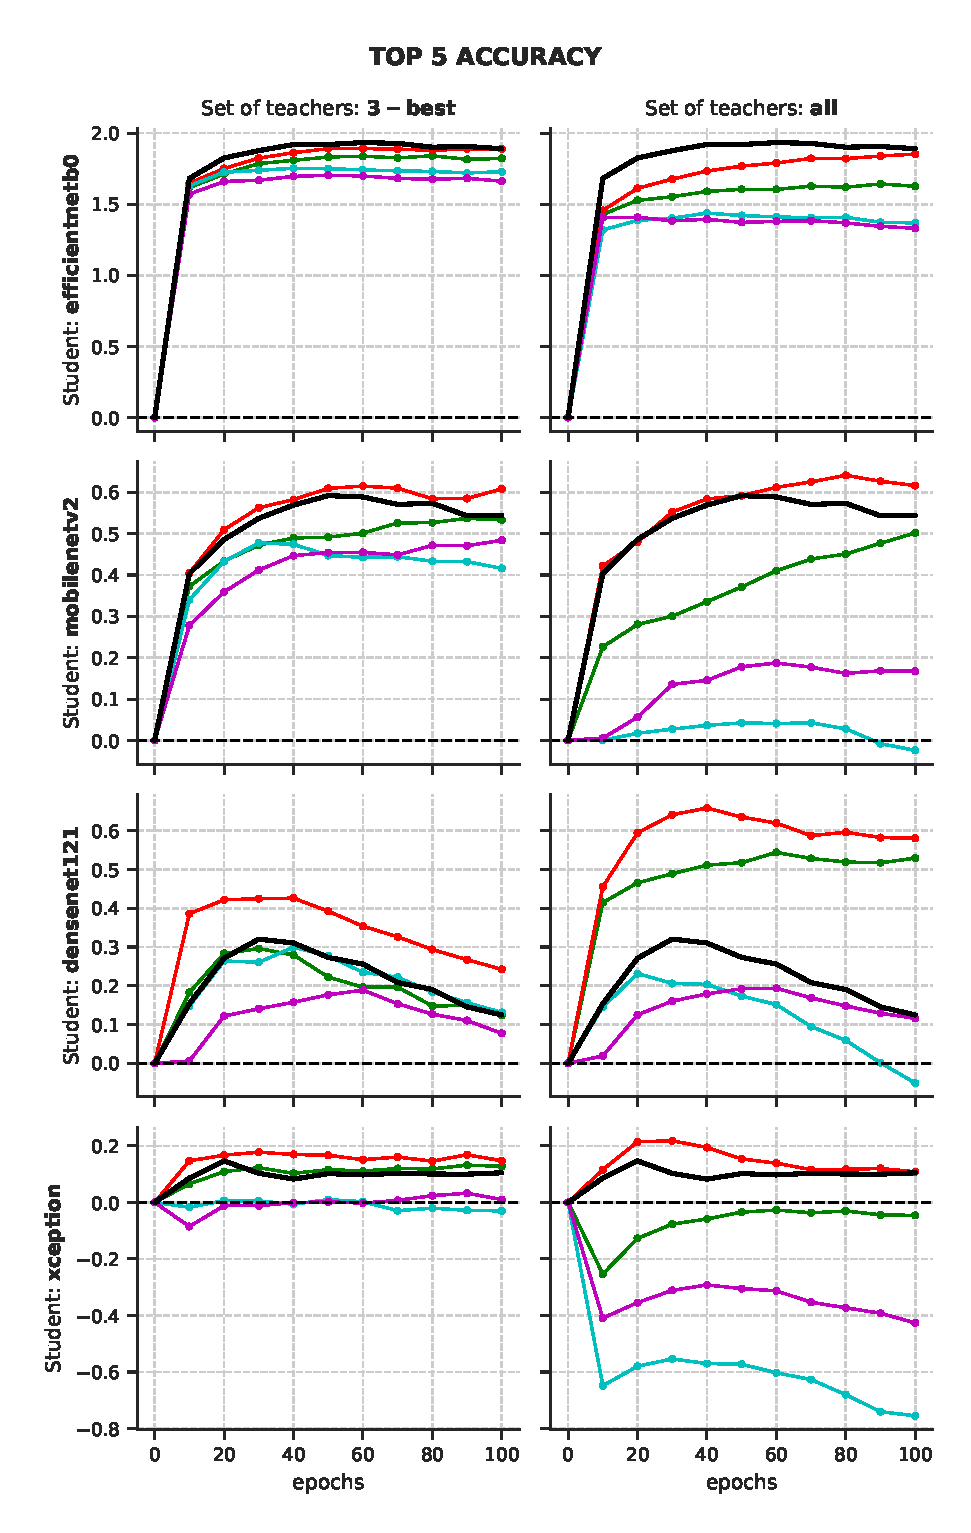
\includegraphics[width=0.475\linewidth]{distillation/images/top5_accuracy_challenging_assumptions}
	 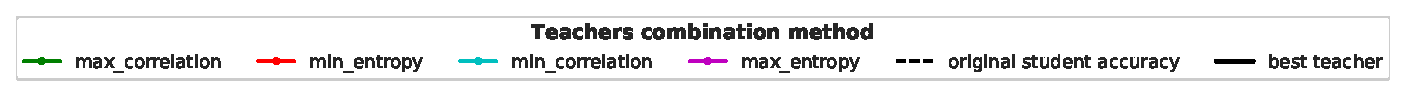
\includegraphics[width=0.95\linewidth]{distillation/images/legend_challenging_assumptions}
	 \caption[Training curves of the min/max entropy and correlation methods]{Absolute difference of top-1 accuracy (left) and top-5 accuracy (right) with respect to the baseline. The x-axis represents the number of training epochs, and the y-axis shows the absolute difference in performance with respect to the baseline. Each row in the grid represents a different student model.}
	 \label{fig:accuracycurves_challenging_assumptions}
 \end{figure}



% Catastrophic forgetting is usually not a problem in pre-trained learning because the target task is different than the original task. It is not the case here.
% Incremental training: parameters of model i are used as initialization for parameters of model i+1
